
\documentclass[
  xcolor={svgnames},
  hyperref={pagebackref,bookmarks},
  aspectratio=169,
  11pt
]{beamer}
\mode<presentation>

% UTDallas-inspired Beamer styling, adapted from the public template structure
\usetheme{Madrid}
\useinnertheme{circles}
\usefonttheme{default}
\setbeamertemplate{navigation symbols}{}

\usepackage[T1]{fontenc}
\usepackage[utf8]{inputenc}
\usepackage{lmodern}
\usepackage{amsmath,amssymb,mathtools}
\usepackage{tikz}
\usetikzlibrary{arrows.meta,positioning,calc,fit,shapes.geometric}
\usepackage{booktabs}
\usepackage{array}
\usepackage{listings}

% UT Dallas palette: orange #E87500, green #053D2C
\definecolor{UTDOrange}{HTML}{E87500}
\definecolor{UTDGreen}{HTML}{053D2C}
\definecolor{UTDSilverleaf}{HTML}{3DA485}
\definecolor{UTDLightOrange}{RGB}{255,239,219}
\definecolor{UTDLightGreen}{RGB}{224,242,235}
\definecolor{UTDLightGray}{RGB}{245,246,244}
\definecolor{UTDDark}{RGB}{30,34,32}

% Backward-compatible color names used by the existing TikZ diagrams
\colorlet{deepblue}{UTDGreen}
\colorlet{softblue}{UTDLightGreen}
\colorlet{softgreen}{UTDLightGreen}
\colorlet{softorange}{UTDLightOrange}
\colorlet{softred}{UTDOrange!13}
\colorlet{softgray}{UTDLightGray}

\setbeamercolor{structure}{fg=UTDOrange}
\setbeamercolor{title}{fg=UTDGreen}
\setbeamercolor{frametitle}{fg=UTDGreen}
\setbeamercolor{normal text}{fg=UTDDark,bg=white}
\setbeamercolor{block title}{fg=white,bg=UTDGreen}
\setbeamercolor{block body}{fg=UTDDark,bg=UTDLightGreen}
\setbeamercolor{alerted text}{fg=UTDOrange}

% Template-style top bar: left section + right current slide title
\providecommand{\insertframetitle}{}
\setbeamertemplate{frametitle}{}
\setbeamerfont{headline}{size=\scriptsize}
\setbeamercolor{headlinebar}{fg=white,bg=UTDGreen}
\setbeamercolor{headlineaccent}{fg=UTDOrange,bg=UTDOrange}
\setbeamertemplate{headline}{%
  \leavevmode%
  \begin{beamercolorbox}[wd=\paperwidth,ht=1.45ex,dp=0.55ex,leftskip=1.0em,rightskip=1.0em]{headlinebar}%
    {\usebeamerfont{headline}\bfseries\insertsectionhead}\hfill{\usebeamerfont{headline}\color{white!85}\insertframetitle}
  \end{beamercolorbox}%
  \begin{beamercolorbox}[wd=\paperwidth,ht=0.22ex,dp=0ex]{headlineaccent}%
  \end{beamercolorbox}%
}

% Template-style footer
\setbeamercolor{footlinebar}{fg=white,bg=UTDGreen}
\setbeamertemplate{footline}{%
  \leavevmode%
  \hbox{%
    \begin{beamercolorbox}[wd=.72\paperwidth,ht=2.35ex,dp=0.9ex,leftskip=1.0em]{footlinebar}%
      \scriptsize\inserttitle
    \end{beamercolorbox}%
    \begin{beamercolorbox}[wd=.18\paperwidth,ht=2.35ex,dp=0.9ex,center]{footlinebar}%
      \scriptsize\insertshortauthor
    \end{beamercolorbox}%
    \begin{beamercolorbox}[wd=.10\paperwidth,ht=2.35ex,dp=0.9ex,center]{footlinebar}%
      \scriptsize\insertframenumber/\inserttotalframenumber
    \end{beamercolorbox}%
  }%
}

\lstset{
  language=Python,
  basicstyle=\ttfamily\small,
  keywordstyle=\color{UTDGreen}\bfseries,
  commentstyle=\color{UTDSilverleaf!75!black},
  stringstyle=\color{UTDOrange!85!black},
  showstringspaces=false,
  columns=fullflexible,
  keepspaces=true,
  backgroundcolor=\color{UTDLightGray},
  frame=single,
  rulecolor=\color{UTDGreen!55},
  frameround=tttt,
  framesep=6pt,
  aboveskip=0.4em,
  belowskip=0.2em
}

\tikzset{
  box/.style={draw=UTDGreen, thick, rounded corners, align=center, fill=UTDLightGreen, minimum height=0.8cm, inner sep=5pt},
  greenbox/.style={draw=UTDGreen, thick, rounded corners, align=center, fill=UTDLightGreen, minimum height=0.8cm, inner sep=5pt},
  orangebox/.style={draw=UTDOrange, thick, rounded corners, align=center, fill=UTDLightOrange, minimum height=0.8cm, inner sep=5pt},
  redbox/.style={draw=UTDOrange!85!black, thick, rounded corners, align=center, fill=UTDOrange!12, minimum height=0.8cm, inner sep=5pt},
  graybox/.style={draw=black!45, thick, rounded corners, align=center, fill=UTDLightGray, minimum height=0.8cm, inner sep=5pt},
  arr/.style={-{Latex[length=3mm]}, thick, draw=UTDGreen},
  darr/.style={-{Latex[length=3mm]}, thick, dashed, draw=UTDOrange!85!black}
}

\title[How microGPT Works]{How microGPT Works}
\subtitle{Number flow, layers, attention, and training motivation}
\author[J Zhao]{J Zhao}
\date{\today}

\begin{document}

\begin{frame}[plain]
\begin{tikzpicture}[remember picture,overlay]
  \fill[white] (current page.south west) rectangle (current page.north east);
  \fill[UTDOrange] (current page.south west) rectangle ([xshift=0.15\paperwidth]current page.north west);
  \fill[UTDGreen] ([xshift=0.15\paperwidth,yshift=-0.055\paperheight]current page.north west) rectangle (current page.north east);
  \fill[UTDGreen] ([xshift=0.15\paperwidth]current page.south west) rectangle ([xshift=0.18\paperwidth]current page.north west);
  \node[rotate=90, text=white, font=\bfseries\Large] at ([xshift=0.075\paperwidth,yshift=0.50\paperheight]current page.south west) {microGPT};
  \node[anchor=west, text=white, font=\bfseries\small] at ([xshift=0.17\paperwidth,yshift=-0.030\paperheight]current page.north west) {UTDallas Beamer style};
  \node[anchor=north east, text=UTDGreen, align=right, font=\bfseries\Huge] at ([xshift=-0.07\paperwidth,yshift=-0.23\paperheight]current page.north east) {How microGPT Works};
  \node[anchor=north east, text=UTDDark, align=right, font=\Large] at ([xshift=-0.07\paperwidth,yshift=-0.36\paperheight]current page.north east) {Number flow, layers, attention,\\and training motivation};
  \node[anchor=south east, text=UTDGreen, align=right, font=\large] at ([xshift=-0.07\paperwidth,yshift=0.10\paperheight]current page.south east) {Study notes};
\end{tikzpicture}
\end{frame}

\section{TOC}
\begin{frame}{Chapter map}
\begin{enumerate}
  \item What the toy GPT is learning
  \item Token IDs, embeddings, and positions
  \item Attention: $Q,K,V$ and weighted retrieval
  \item Transformer layer interpretation
  \item Prediction, loss, and Adam update
  \item Motivation: why these strange formulas exist
\end{enumerate}
\end{frame}

% ---------------- Chapter 1 ----------------
\section{What the toy GPT is learning}
\begin{frame}{Chapter 1 - The model is a name generator}
The code trains a character-level autoregressive model.

\vspace{0.4cm}
For a name like \texttt{emma}, the sequence is
\[
[\mathrm{BOS},e,m,m,a,\mathrm{BOS}].
\]

The model learns conditional probabilities with a finite context window $B=\texttt{block\_size}$:
\[
P_\theta\!\left(x_{t+1}\mid x_{\max(0,t-B+1)},\ldots,x_t\right).
\]

Here $T$ is the number of prediction steps for one example. For a name with $n$ characters, $T=n+1$ because the final BOS/end token is also predicted.

A full name probability is factored as
\[
P_\theta(x_1,\ldots,x_T)=\prod_{t=0}^{T-1}P_\theta\!\left(x_{t+1}\mid x_{\max(0,t-B+1)},\ldots,x_t\right).
\]
\end{frame}

\begin{frame}{The whole pipeline}
\centering
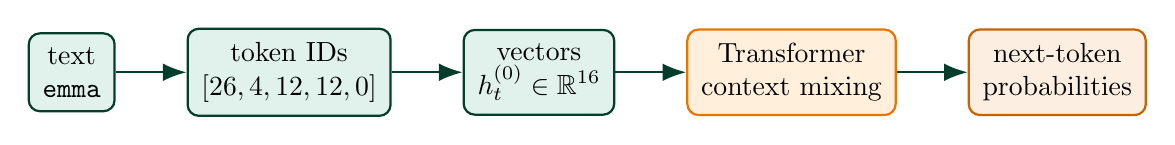
\begin{tikzpicture}[node distance=0.9cm]
\node[box] (txt) {text\\\texttt{emma}};
\node[box, right=of txt] (ids) {token IDs\\$[26,4,12,12,0]$};
\node[greenbox, right=of ids] (emb) {vectors\\$h_t^{(0)}\in\mathbb R^{16}$};
\node[orangebox, right=of emb] (tr) {Transformer\\context mixing};
\node[redbox, right=of tr] (prob) {next-token\\probabilities};
\draw[arr] (txt)--(ids);
\draw[arr] (ids)--(emb);
\draw[arr] (emb)--(tr);
\draw[arr] (tr)--(prob);
\end{tikzpicture}

\vspace{0.45cm}
\[
h_t^{(\ell)}=\text{hidden vector at position }t\text{ after layer }\ell.
\]
\[
h_t^{(0)}=E_{\rm tok}[x_t]+E_{\rm pos}[t].
\]
\vspace{-0.1cm}
\[
\text{discrete text}\longrightarrow \text{fixed IDs}\longrightarrow \text{learned vectors}\longrightarrow \text{probabilities}.
\]
\end{frame}

% ---------------- Chapter 2 ----------------
\section{Token IDs, embeddings, and positions}
\begin{frame}[fragile]{Chapter 2 - Token IDs are fixed; embeddings are learned}
The tokenizer gives fixed IDs:
\[
a\mapsto 0,\quad b\mapsto 1,\quad\ldots,\quad z\mapsto 25,\quad \mathrm{BOS}\mapsto 26.
\]

The token embedding matrix is learned:
\[
E_{\mathrm{tok}}\in\mathbb R^{27\times 16}.
\]

If \texttt{m} has ID $12$, then
\[
E_{\mathrm{tok}}[m]=E_{\mathrm{tok}}[12,:]\in\mathbb R^{16}.
\]

Initialization:
\[
E_{\rm tok}[i,j]\sim\mathcal N(0,0.08^2).
\]
\begin{center}
\begin{minipage}{0.84\linewidth}
\begin{lstlisting}
matrix = lambda nout, nin, std=0.08: [
    [Value(random.gauss(0, std)) for _ in range(nin)]
    for _ in range(nout)
]
state_dict['wte'] = matrix(vocab_size, n_embd)
\end{lstlisting}
\end{minipage}
\end{center}
\end{frame}

\begin{frame}{One-hot view versus embedding lookup}
\centering
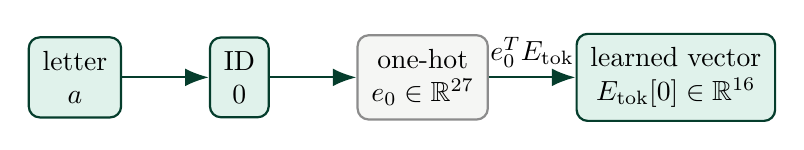
\begin{tikzpicture}[node distance=1.1cm]
\node[box] (letter) {letter\\$a$};
\node[box, right=of letter] (id) {ID\\$0$};
\node[graybox, right=of id] (onehot) {one-hot\\$e_0\in\mathbb R^{27}$};
\node[greenbox, right=of onehot] (emb) {learned vector\\$E_{\rm tok}[0]\in\mathbb R^{16}$};
\draw[arr] (letter)--(id);
\draw[arr] (id)--(onehot);
\draw[arr] (onehot)--node[above] {$e_0^T E_{\rm tok}$} (emb);
\end{tikzpicture}

\vspace{0.35cm}
\[
\boxed{\text{one-hot vector}=\text{a standard basis vector }e_i}
\]
Every one-hot vector is a unit vector, but not every unit vector is one-hot. The code directly performs the row lookup.
\end{frame}

\begin{frame}{Position embeddings}
Define
\[
\boxed{d:=\text{embedding dimension}=\texttt{n\_embd}=16.}
\]
The position embedding matrix is also learned:
\[
E_{\mathrm{pos}}\in\mathbb R^{B\times d}.
\]
In this toy code,
\[
B=16,\qquad d=16,
\]
so
\[
E_{\mathrm{pos}}\in\mathbb R^{16\times16}.
\]
This square shape is accidental: context length and embedding width both happen to be 16.
\end{frame}

\begin{frame}{Example: positions in \texttt{emma}}
For \texttt{emma}, the input positions are:
\[
\begin{array}{c|c|c}
\text{position }t & \text{input token} & \text{target token}\\\hline
0 & \mathrm{BOS} & e\\
1 & e & m\\
2 & m & m\\
3 & m & a\\
4 & a & \mathrm{BOS}
\end{array}
\]

The first \texttt{m} has representation
\[
h_2^{(0)}=E_{\mathrm{tok}}[m]+E_{\mathrm{pos}}[2].
\]
The second \texttt{m} uses the same token embedding but a different position vector:
\[
h_3^{(0)}=E_{\mathrm{tok}}[m]+E_{\mathrm{pos}}[3].
\]
\end{frame}

\begin{frame}{Why add token and position vectors?}
The model needs one $d$-dimensional vector containing both identity and position:
\[
h_t^{(0)}=E_{\mathrm{tok}}[x_t]+E_{\mathrm{pos}}[t].
\]
\[
\boxed{\text{Addition is not sacred. It is cheap and keeps dimension fixed.}}
\]

\vspace{0.3cm}
A more literal alternative would be concatenation:
\[
\begin{bmatrix}E_{\mathrm{tok}}[x_t]\\E_{\mathrm{pos}}[t]\end{bmatrix}\in\mathbb R^{2d}.
\]
But that widens the model or requires another projection.
\end{frame}

% ---------------- Chapter 3 ----------------
\section{Attention}
\begin{frame}{Chapter 3 - From hidden vector to Q, K, V}
At each position, the vector is first normalized:
\[
\tilde h_t=\operatorname{RMSNorm}(h_t).
\]
Then three learned linear maps are applied:
\[
q_t=W_Q\tilde h_t,\qquad k_t=W_K\tilde h_t,\qquad v_t=W_V\tilde h_t.
\]
Here
\[
W_Q,W_K,W_V\in\mathbb R^{16\times16}.
\]

They are structurally similar, but their roles differ in the attention formula.
\end{frame}

\begin{frame}{Q, K, V roles}
\centering
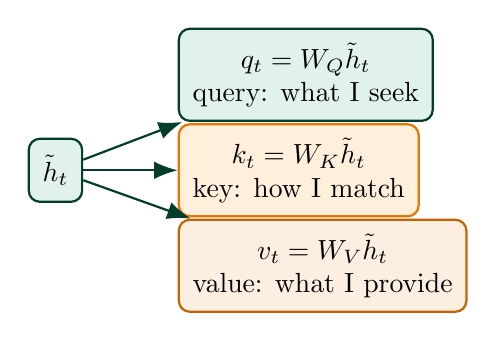
\begin{tikzpicture}[node distance=1.1cm]
\node[box] (x) {$\tilde h_t$};
\node[greenbox, above right=0.2cm and 1.2cm of x] (q) {$q_t=W_Q\tilde h_t$\\query: what I seek};
\node[orangebox, right=1.2cm of x] (k) {$k_t=W_K\tilde h_t$\\key: how I match};
\node[redbox, below right=0.2cm and 1.2cm of x] (v) {$v_t=W_V\tilde h_t$\\value: what I provide};
\draw[arr] (x)--(q);
\draw[arr] (x)--(k);
\draw[arr] (x)--(v);
\end{tikzpicture}

\vspace{0.5cm}
$Q,K$ decide routing. $V$ supplies the routed content.
\end{frame}

\begin{frame}{Attention score and output}
For head dimension
\[
d_h=\frac{d}{H}=\frac{16}{4}=4,
\]
the score from current position $t$ to source position $s$ is
\[
s_{ts}^{(h)}=\frac{(q_t^{(h)})^T k_s^{(h)}}{\sqrt{d_h}}.
\]
Softmax gives weights:
\[
\alpha_{ts}^{(h)}=\frac{e^{s_{ts}^{(h)}}}{\sum_{r\le t}e^{s_{tr}^{(h)}}}.
\]
The head output is
\[
o_t^{(h)}=\sum_{s\le t}\alpha_{ts}^{(h)}v_s^{(h)}.
\]
\end{frame}

\begin{frame}{Attention as differentiable retrieval}
\centering
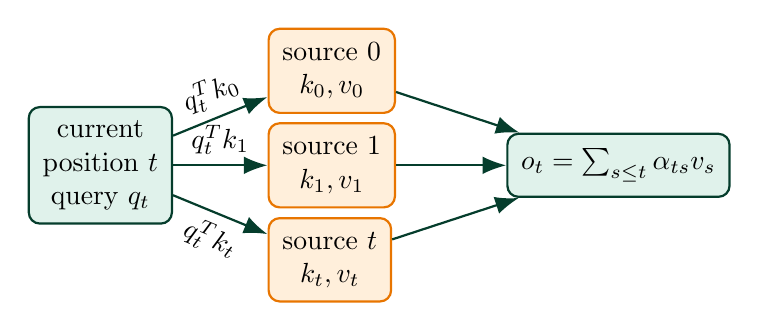
\begin{tikzpicture}[node distance=0.75cm]
\node[box] (cur) {current\\position $t$\\query $q_t$};
\node[orangebox, right=1.2cm of cur, yshift=1.2cm] (s0) {source $0$\\$k_0,v_0$};
\node[orangebox, right=1.2cm of cur] (s1) {source $1$\\$k_1,v_1$};
\node[orangebox, right=1.2cm of cur, yshift=-1.2cm] (s2) {source $t$\\$k_t,v_t$};
\node[greenbox, right=1.4cm of s1] (out) {$o_t=\sum_{s\le t}\alpha_{ts}v_s$};
\draw[arr] (cur)--node[above, sloped] {$q_t^Tk_0$} (s0);
\draw[arr] (cur)--node[above] {$q_t^Tk_1$} (s1);
\draw[arr] (cur)--node[below, sloped] {$q_t^Tk_t$} (s2);
\draw[arr] (s0)--(out);
\draw[arr] (s1)--(out);
\draw[arr] (s2)--(out);
\end{tikzpicture}
\end{frame}

\begin{frame}{Matrix form of attention}
Ignoring transpose conventions, attention is usually written as
\[
Q=XW_Q,\qquad K=XW_K,\qquad V=XW_V.
\]
The attention operation is
\[
\operatorname{Attention}(Q,K,V)
=
\operatorname{softmax}\left(\frac{QK^T}{\sqrt{d_h}}\right)V.
\]

\vspace{0.3cm}
In the code, vectors are handled one position at a time with a key-value cache. The mathematics is the same causal version:
\[
s\le t.
\]
\end{frame}

% ---------------- Chapter 4 ----------------
\section{Transformer layer interpretation}
\begin{frame}{Chapter 4 - One Transformer layer}
This toy GPT has
\[
\texttt{n\_layer}=1.
\]
That one Transformer layer contains:
\begin{enumerate}
  \item RMSNorm before attention
  \item multi-head causal attention
  \item output projection $W_O$
  \item residual addition
  \item RMSNorm before MLP
  \item two-linear-layer MLP: $W_2\operatorname{ReLU}(W_1x)$
  \item residual addition
\end{enumerate}
For the MLP, define $d_{\rm ff}=rd$, where $r$ is the expansion-ratio hyperparameter. Here $r=4$, independent of the number of attention heads $H$.
\end{frame}

\begin{frame}{Layer diagram}
\centering
\resizebox{!}{0.72\textheight}{%
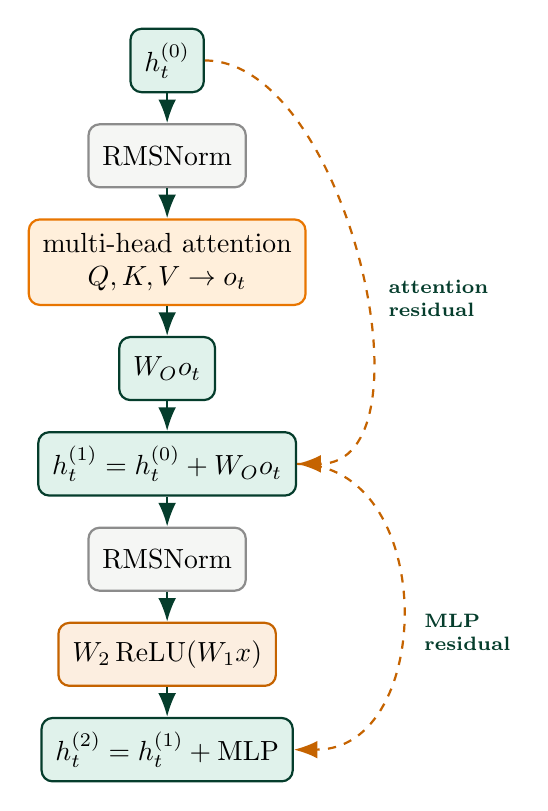
\begin{tikzpicture}[node distance=0.38cm, transform shape]
\node[box] (h0) {$h_t^{(0)}$};
\node[graybox, below=of h0] (n1) {RMSNorm};
\node[orangebox, below=of n1] (att) {multi-head attention\\$Q,K,V \to o_t$};
\node[box, below=of att] (wo) {$W_Oo_t$};
\node[greenbox, below=of wo] (res1) {$h_t^{(1)}=h_t^{(0)}+W_Oo_t$};
\node[graybox, below=of res1] (n2) {RMSNorm};
\node[redbox, below=of n2] (mlp) {$W_2\operatorname{ReLU}(W_1x)$};
\node[greenbox, below=of mlp] (res2) {$h_t^{(2)}=h_t^{(1)}+\mathrm{MLP}$};
\draw[arr] (h0)--(n1);
\draw[arr] (n1)--(att);
\draw[arr] (att)--(wo);
\draw[arr] (wo)--(res1);
\draw[arr] (res1)--(n2);
\draw[arr] (n2)--(mlp);
\draw[arr] (mlp)--(res2);
\draw[darr] (h0.east) .. controls +(1.8,0) and +(1.8,0) .. node[pos=0.56, right=0.18cm, align=left, text=deepblue, font=\scriptsize\bfseries] {attention\\residual} (res1.east);
\draw[darr] (res1.east) .. controls +(1.8,0) and +(1.8,0) .. node[pos=0.56, right=0.18cm, align=left, text=deepblue, font=\scriptsize\bfseries] {MLP\\residual} (res2.east);
\end{tikzpicture}%
}
\end{frame}


\begin{frame}{How attention heads are concatenated}
Each head returns a vector of dimension
\[
d_h=\frac{d}{H}.
\]
In this microGPT,
\[
d=16,\qquad H=4,\qquad d_h=4.
\]
So the four head outputs are
\[
o_t^{(1)},o_t^{(2)},o_t^{(3)},o_t^{(4)}\in\mathbb R^4.
\]
They are joined by concatenation:
\[
o_t=
\operatorname{Concat}\!\left(o_t^{(1)},o_t^{(2)},o_t^{(3)},o_t^{(4)}\right)
\in\mathbb R^{4\cdot4}=\mathbb R^{16}.
\]
Then the output projection mixes the four coordinate blocks:
\[
a_t=W_Oo_t.
\]
\end{frame}

\begin{frame}{$W_O$, $W_1$, and $W_2$}
After the heads are concatenated,
\[
o_t\in\mathbb R^{16}.
\]
The output projection mixes heads:
\[
a_t=W_Oo_t,\qquad W_O\in\mathbb R^{16\times16}.
\]
The MLP is
\[
\operatorname{MLP}(x)=W_2\operatorname{ReLU}(W_1x).
\]
Let $d_{\rm ff}=rd$ with expansion ratio $r=4$:
\[
W_1\in\mathbb R^{rd\times d}=\mathbb R^{64\times16},\qquad
W_2\in\mathbb R^{d\times rd}=\mathbb R^{16\times64}.
\]
\[
\boxed{r=4\text{ is independent of the number of attention heads }H.}
\]
\end{frame}

% ---------------- Chapter 5 ----------------
\section{Prediction, loss, and Adam}
\begin{frame}{Chapter 5 - Output prediction}
The final hidden vector is
\[
h_t^{(2)}\in\mathbb R^{16}.
\]
The output matrix is learned:
\[
W_{\mathrm{out}}\in\mathbb R^{27\times16}.
\]
It produces logits:
\[
\ell_t=W_{\mathrm{out}}h_t^{(2)}\in\mathbb R^{27}.
\]
\[
\boxed{\text{logits are raw, unnormalized scores before softmax.}}
\]
Each coordinate $\ell_{t,i}$ is the raw score for token $i$.

Softmax produces probabilities:
\[
p_{t,j}=\frac{e^{\ell_{t,j}}}{\sum_{k=0}^{26}e^{\ell_{t,k}}}.
\]
$W_{\mathrm{out}}$ is a parameter. $p_t$ is the prediction.
\end{frame}

\begin{frame}{Loss: negative log-likelihood}
The target is a discrete token ID:
\[
\boxed{y_t=x_{t+1}\in\{0,\ldots,V-1\}.}
\]
It is not a vector; its embedding would be $E_{\rm tok}[y_t]\in\mathbb R^d$.
The loss at position $t$ is
\[
L_t=-\log p_{t,y_t}.
\]
For the full sequence,
\[
L(\theta)=-\frac{1}{T}\sum_{t=0}^{T-1}\log P_\theta\!\left(x_{t+1}\mid x_{\max(0,t-B+1)},\ldots,x_t\right).
\]
Here $T$ is the number of prediction steps; for a name with $n$ characters, $T=n+1$.
This is cross-entropy / negative log-likelihood.

\vspace{0.3cm}
It is small when the model assigns high probability to the observed next token.
\end{frame}

\begin{frame}{Parameter space}
All learned matrices are part of $\theta$:
\[
\theta=\{E_{\rm tok},E_{\rm pos},W_Q,W_K,W_V,W_O,W_1,W_2,W_{\rm out}\}.
\]
For this toy model,
\[
\boxed{\dim(\Theta)=\underbrace{2Vd}_{E_{\rm tok}+W_{\rm out}}+\underbrace{Bd}_{E_{\rm pos}}+\underbrace{12Ld^2}_{\text{attention and MLP matrices}}.}
\]
For one Transformer layer,
\[
\boxed{12d^2=\underbrace{4d^2}_{W_Q,W_K,W_V,W_O}+\underbrace{8d^2}_{W_1,W_2}.}
\]
The MLP part is $8d^2=4d^2+4d^2$ because $W_1\in\mathbb R^{4d\times d}$ and $W_2\in\mathbb R^{d\times4d}$.

With $V=27, B=16, d=16, L=1$:
\[
2(27)(16)+16(16)+12(1)(16^2)=4192,
\qquad \Theta=\mathbb R^{4192}.
\]
\end{frame}

\begin{frame}{Adam update}
For each parameter coordinate, let
\[
g_t=\frac{\partial L_t}{\partial\theta}.
\]
Adam keeps two running estimates:
\[
m_t=\beta_1m_{t-1}+(1-\beta_1)g_t,
\]
\[
v_t=\beta_2v_{t-1}+(1-\beta_2)g_t^2.
\]
Bias correction:
\[
\hat m_t=\frac{m_t}{1-\beta_1^t},\qquad
\hat v_t=\frac{v_t}{1-\beta_2^t}.
\]
Update:
\[
\theta_t=\theta_{t-1}-\eta_t\frac{\hat m_t}{\sqrt{\hat v_t}+\varepsilon}.
\]
\end{frame}

% ---------------- Chapter 6 ----------------
\section{Motivation}
\begin{frame}{Chapter 6 - Why attention?}
The old bottleneck: compress the whole previous sequence into one state.
\[
h_t=f(h_{t-1},x_t).
\]
Attention avoids this by keeping all previous position representations and retrieving selectively:
\[
o_t=\sum_{s\le t}\alpha_{ts}v_s.
\]
The central idea:
\[
\boxed{\text{do not memorize everything in one vector; retrieve what is relevant.}}
\]
\end{frame}

\begin{frame}{Why query, key, and value?}
The model must answer two questions:
\[
\text{Where should I look?}
\]
\[
\text{What information should I take?}
\]

So it separates matching from content:
\[
q_t=W_Qx_t\quad\text{request},
\]
\[
k_s=W_Kx_s\quad\text{index},
\]
\[
v_s=W_Vx_s\quad\text{content}.
\]
Then
\[
\alpha_{ts}=\operatorname{softmax}_s\left(\frac{q_t^Tk_s}{\sqrt{d_h}}\right),
\qquad
 o_t=\sum_s\alpha_{ts}v_s.
\]
\end{frame}

\begin{frame}{Why dot product and softmax?}
The dot product is a cheap compatibility score:
\[
q_t^Tk_s=\|q_t\|\,\|k_s\|\cos\theta.
\]
In matrix form, all pairwise scores are computed by
\[
QK^T.
\]
Softmax converts arbitrary scores into differentiable selection weights:
\[
\alpha_s=\frac{e^{s_s}}{\sum_r e^{s_r}}.
\]
It is a smooth version of choosing the most relevant source.
\end{frame}

\begin{frame}{Why divide by $\sqrt{d_h}$?}
If coordinates of $q$ and $k$ have roughly unit variance, then
\[
q^Tk=\sum_{j=1}^{d_h}q_jk_j
\]
has variance about
\[
\operatorname{Var}(q^Tk)\approx d_h.
\]
So the typical scale grows like $\sqrt{d_h}$.

Dividing by $\sqrt{d_h}$ keeps score magnitudes stable:
\[
\frac{q^Tk}{\sqrt{d_h}}.
\]
This prevents softmax from saturating too early and improves gradients.
\end{frame}

\begin{frame}{Why multiple heads and an MLP?}
Multiple heads allow several retrieval patterns in parallel:
\[
o_t=o_t^{(1)}\Vert o_t^{(2)}\Vert\cdots\Vert o_t^{(H)}.
\]
Then $W_O$ mixes the head outputs.

\vspace{0.4cm}
Attention communicates across positions:
\[
\boxed{\text{which previous information matters?}}
\]
The MLP performs nonlinear computation at each position:
\[
\boxed{\text{how should the gathered information be transformed?}}
\]
\end{frame}

\begin{frame}{One-sentence summary}
\centering
\Large
\[
\boxed{
\begin{gathered}
\text{Embeddings create token-position vectors.}\\
\text{Attention retrieves relevant previous information.}\\
\text{The MLP transforms it nonlinearly.}\\
\text{The output head turns it into next-token probabilities.}
\end{gathered}}
\]
\end{frame}


% ---------------- Appendix ----------------
\appendix
\section{Appendix A: mathematical notation versus code notation}
\begin{frame}{Appendix A - Mathematical notation versus code notation}
\small
\[
h_t^{(\ell)}\leftrightarrow \texttt{x},\qquad
 t\leftrightarrow\texttt{pos\_id},\qquad
 \ell\leftrightarrow\texttt{li}.
\]
\begin{center}
\begin{tabular}{ll}
\toprule
Mathematics & Code \\
\midrule
$E_{\rm tok}$ & \texttt{state\_dict['wte']} \\
$E_{\rm pos}$ & \texttt{state\_dict['wpe']} \\
$W_Q$ & \texttt{state\_dict[f'layer\{li\}.attn\_wq']} \\
$W_K$ & \texttt{state\_dict[f'layer\{li\}.attn\_wk']} \\
$W_V$ & \texttt{state\_dict[f'layer\{li\}.attn\_wv']} \\
$W_O$ & \texttt{state\_dict[f'layer\{li\}.attn\_wo']} \\
$W_1$ & \texttt{state\_dict[f'layer\{li\}.mlp\_fc1']} \\
$W_2$ & \texttt{state\_dict[f'layer\{li\}.mlp\_fc2']} \\
$W_{\rm out}$ & \texttt{state\_dict['lm\_head']} \\
\bottomrule
\end{tabular}
\end{center}
The code reuses \texttt{x}; the mathematical notation keeps layer and position explicit.
\end{frame}

\section{Appendix B: why the initialization scale is 0.08}
\begin{frame}[fragile]{Appendix B - Why the initialization scale is $0.08$}
\small
The entries are initialized as
\[
E_{\rm tok}[i,j]\sim\mathcal N(0,0.08^2).
\]
The value $0.08$ is a heuristic, not a mathematical constant. It breaks symmetry while keeping early activations, attention scores, and gradients moderate.
\begin{itemize}
  \item Too large: dot products $q^Tk$ may be large, making softmax too sharp.
  \item Too small: signals and gradients may be weak.
  \item More systematic alternatives include Xavier and He initialization.
\end{itemize}
\begin{lstlisting}
matrix = lambda nout, nin, std=0.08: [
    [Value(random.gauss(0, std)) for _ in range(nin)]
    for _ in range(nout)
]
\end{lstlisting}
\end{frame}

\section{Appendix C: RMSNorm}
\begin{frame}{Appendix C - RMSNorm}
\small
For $x\in\mathbb R^d$,
\[
\operatorname{RMS}(x)=\sqrt{\frac1d\sum_{i=1}^d x_i^2+\varepsilon}.
\]
General RMSNorm is
\[
\operatorname{RMSNorm}_g(x)=g\odot\frac{x}{\operatorname{RMS}(x)}.
\]
Residual additions can cause scale drift:
\[
x\leftarrow x+\operatorname{Attention}(x),\qquad x\leftarrow x+\operatorname{MLP}(x).
\]
RMSNorm stabilizes attention-score and MLP-input magnitudes. Unlike LayerNorm, it does not subtract the mean.
\[
\boxed{\text{RMSNorm stabilizes the scale of hidden vectors before learned transformations.}}
\]
\end{frame}

\section[Appendix D: RMSNorm gain]{Appendix D: learned versus fixed RMSNorm gain $g$}
\begin{frame}[fragile]{Appendix D - Learned versus fixed RMSNorm gain $g$}
\small
Standard RMSNorm usually learns
\[
g\in\mathbb R^d,
\qquad g_i=1\text{ at initialization.}
\]
\[
\boxed{\text{fixed }g=\mathbf1:\text{ normalization only}}
\qquad
\boxed{\text{learned }g:\text{ normalization plus coordinatewise rescaling}}
\]
This microGPT fixes $g=\mathbf1$ implicitly, so $g$ is not a trainable parameter in the actual code.
\begin{lstlisting}
def rmsnorm(x):                 # actual microGPT version
    ms = sum(xi * xi for xi in x) / len(x)
    scale = (ms + 1e-5) ** -0.5
    return [xi * scale for xi in x]

# learned-gain version would use:
# return [gi * xi * scale for xi, gi in zip(x, gain)]
\end{lstlisting}
Fixing $g$ is valid for a tiny model; learned $g$ usually improves flexibility at negligible cost.
\end{frame}

\section[Appendix E: Q/K/V dimensions]{Appendix E: dimensions of $Q$, $K$, and $V$}
\begin{frame}{Appendix E - Dimensions of $Q$, $K$, and $V$}
\small
For each attention head,
\[
q_t,k_t,v_t\in\mathbb R^{d_h},\qquad d_h=\frac dH.
\]
For microGPT,
\[
d=16,\qquad H=4,\qquad d_h=4.
\]
Thus each head uses
\[
q_t,k_t,v_t\in\mathbb R^4.
\]
Across all heads,
\[
Hd_h=d=16.
\]
\[
\boxed{d\text{ determines the total }Q,K,V\text{ dimension, while }d_h=d/H\text{ is the dimension per head.}}
\]
\end{frame}

\section[Appendix F: MLP formula]{Appendix F: mathematical form of the MLP}
\begin{frame}{Appendix F - Mathematical form of $W_2\operatorname{ReLU}(W_1x)$}
\small
\[
\operatorname{MLP}(x)=W_2\operatorname{ReLU}(W_1x),
\]
where
\[
x\in\mathbb R^d,
\quad W_1\in\mathbb R^{d_{\rm ff}\times d},
\quad W_2\in\mathbb R^{d\times d_{\rm ff}}.
\]
For microGPT,
\[
d=16,
\qquad d_{\rm ff}=64.
\]
Let
\[
z=W_1x\in\mathbb R^{64},\qquad \operatorname{ReLU}(z)_i=\max(0,z_i),
\]
then
\[
y=W_2\operatorname{ReLU}(z)\in\mathbb R^{16}.
\]
Coordinate form:
\[
y_i=\sum_{j=1}^{64}(W_2)_{ij}\max\left(0,\sum_{k=1}^{16}(W_1)_{jk}x_k\right).
\]
\[
\boxed{W_1\text{ expands }16\to64,\quad \operatorname{ReLU}\text{ adds nonlinearity},\quad W_2\text{ compresses }64\to16.}
\]
\end{frame}

\end{document}
